\chapter{Architektur und verwendete Technologien}\label{ch:architektur-und-verwendete-technologien}


\section{Architektur}\label{sec:architektur}
Die Applikation besteht aus zwei klar getrennten Teilen, die unabhängig voneinander funktionieren.
Das Backend kann also mit beliebigen Frontends (z.B. Web-Clients, Apps oder Postman) verwendet werden.
Folgend sind die beiden Komponenten kurz beschrieben.

\begin{center}
   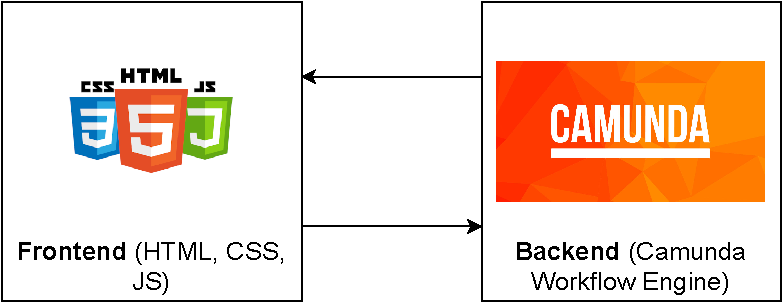
\includegraphics[width=1\textwidth]{resources/architecture}
\end{center}


\begin{description}
   \item[Backend (Camunda Workflow Engine)] Den Kern der Applikation bildet die Camunda Workflow Engine, bzw. der Kaffemaschinen--Prozess, der darauf deployed ist.
   Das Backend stellt die funktionsfähige Kaffeemaschine dar und hält die aktuellen Füllstände sowie den Zustand, in dem sich die Maschine aktuell befindet.
   Sobald der Prozess einmal gestartet wurde, ist die Machine bereit für die Verwendung.
   Das Backend bzw. die Maschine wird über eine REST-API gesteuert werden.
   Die Endpoints sind im Abschnitt~\ref{sec:endpoints} beschrieben.
   \item[Frontend (HTML, CSS, JS)] Das Frontend stellt eine grafische Benutzeroberfläche für die Kaffeemaschine zur Verfügung.
   Über die REST-API werden Informationen wie z.B. die aktuellen Füllstände oder den Status vom Backend abgerufen und im Frontend dargestellt.
   Weiter werden die Steuerungsbefehle des Benutzers, wie das Ein- und Ausschalten der Maschine oder das Nachfüllen eines Behälters an das Backend übertragen.
\end{description}


\section{Endpoints}\label{sec:endpoints}
Die folgende Tabelle bietet eine Übersicht über die verfügbaren Endpoints der REST-API.

\begin{longtable}{|p{.15\textwidth}|p{.15\textwidth}|p{.20\textwidth}|p{.50\textwidth}|}
   \hline
   \textbf{Methode} &\textbf{Endpoint} & \textbf{Beschreibung} & \textbf{Body Content} \\ \hline
   POST & /message & Maschine einschalten
   & \begin{minted}{json}
   {"messageName": "power_on"}
   \end{minted}
   \\ \hline
   /POST & message
   & Maschine ausschalten
   & \begin{minted}{json}
   {"messageName": "power_off"}
   \end{minted}
   \\ \hline
   /POST & message
   & Bohnen auffüllen
   & \begin{minted}{json}
   {"messageName": "fill_beans"}
   \end{minted}
   \\ \hline
   /POST & message
   & Wasser auffüllen
   & \begin{minted}{json}
   {"messageName": "fill_water"}
   \end{minted}
   \\ \hline
   /POST & message
   & Milch auffüllen
   & \begin{minted}{json}
   {"messageName": "fill_milk"}
   \end{minted}
   \\ \hline
   /POST & message
   & Zucker auffüllen
   & \begin{minted}{json}
   {"messageName": "fill_sugar"}
   \end{minted}
   \\ \hline
   /POST & message
   & Kaffe herauslassen
   & \begin{minted}{json}
   {
      "messageName": "selection",
      "processVariables": {
         "type": {
            "type": "string",
            "value": "mokka"
         }
      }
   }
   \end{minted}
   \\ \hline
   GET & /process-instance/<id>/variables/levels
   & Füllstände abfragen
   & --
   \\ \hline
   GET & /process-instance/<id>/variables/display
   & Aktueller Wert des Displays abfragen
   & --
   \\ \hline
\end{longtable}\label{tab:endpoints}


\section{Technologien}\label{sec:technologien}
In der folgenden Tabelle sind die Technologien aufgeführt, die wir in unserem Projekt verwenden.

\begin{longtable}{|p{.50\textwidth}|p{.50\textwidth}|}
   \hline
   \textbf{Technologie/Software} & \textbf{Verwendung}
   \\ \hline
   Camunda Modeler & Zeichnen der Diagramme.
   \\ \hline
   Camunda Workflow Engine & Backend der Applikation.
   Führt die definierten Prozesse aus.
   \\ \hline
   Docker
   & Die Workflow Engine läuft in einem Docker Container.
   \\ \hline
   HTML, CSS, JavaScript
   & Für das Frontend verwendet.
   \\ \hline
   Postman
   & Testen der Backend-API.
   \\ \hline
\end{longtable}\label{tab:technologies}
